\section{Переход к турбулентности путем удвоения периодов  \texorpdfstring{($\S 32$)}{Lg}}

Отдельно можно рассмотреть потерю устойчивости периодическим движением путём прохождения мультипликатора через значения $-1$ или $+1$.

В $n$-мерном пространстве состояний $n-1$ мультипликаторов 
определяют поведение траекторий в $n - 1$ различных направлениях в окрестности рассматриваемой периодической траектории 
(отличных от направления касательной в каждой точке самой 
этой траектории). Пусть близкий к $\pm 1$ мультипликатор отвечает некоторому 1-му направлению. Остальные $n - 2$ мультипликаторов малы по модулю; поэтому по соответствующим им 
$n - 2$ направлениям все траектории будут со временем прижиматься к некоторой двумерной поверхности (назовем ее $\Sigma$), которой принадлежат 1-е направление и направление указанных касательных. Можно сказать, что в окрестности предельного цикла 
пространство состояний при $t \to \infty$ оказывается почти двумерным (строго двумерным оно не может быть -- траектории могут 
располагаться по обе стороны $S$ и переходить с одной стороны 
поверхности на другую). 


\subsection{Отображение Пуанкаре}
Разрежем поток траекторий вблизи $S$ некоторой секущей поверхностью $\sigma$. 
Каждая траектория, повторно пересекая $\sigma$, ставит в соответствие исходной точке пересечения (назовем ее $\vc{x}_j$) точку пересечения в момент следующего возврата $\vc{x}_{j+1}$. Связь $\vc{x}_{j+1} = f (\vc{x}_j:R)$ называют \textbf{отображением Пуанкаре} (или отображением последования); она зависит от параметра $R$ (в данном случае -- числа Рейнольдса), значение которого определяет степень близости к бифуркации -- потере 
устойчивости периодическим движением. 
Поскольку все траектории тесно прижаты к поверхности $\Sigma$, множество точек пересечения поверхности $\sigma$ траекториями оказывается почти одномерным, и его можно приближенно аппроксимировать линией; 
отображение Пуанкаре станет одномерным преобразованием: $x_{j+1} = f(x_j;R)$, причём $x$ будет просто координатой на указанной линии. Дискретная переменная $j$ играет роль времени, измеряемого в единицах периода движения.

Одномерное отображение Пуанкаре дает альтернативный способ определения характера течения вблизи бифуркации. 
Самому периодическому движению отвечает \textbf{неподвижная точка} -- значение $x_j = x_*$, не меняющееся при отображении, то есть для которого $x_{j+1} = x_j$. 
Роль мультипликатора играет производная $\mu = \d x_{j+1}/\d x_j$, взятая в неподвижной точке. Точки $x_j = x_* + \xi$ в окрестности $x_*$ в результате отображения переходят в $x_{j+1} \approx x_* + \mu \xi$. 
Неподвижная точка устойчива (и является аттрактором отображения), если $|\mu| < 1$: повторно применяя отображение и начав с какой-либо точки в окрестности точки $x_*$, мы будем асимптотически приближаться к последней (по закону $\mu^j$, где $j$— число итераций). Напротив, при $|\mu| > 1$ неподвижная точка неустойчива. 


\subsection{Бифуркация удвоения периода}
Рассмотрим потерю устойчивости периодическим движением при переходе мультипликатора через $-1$. Равенство $\mu = -1$ означает, что начальное возмущение через интервал времени $T_0$ меняет знак, не меняясь по абсолютной величине: еще через период $T_0$ возмущение перейдет само в себя. 
Таким образом, при переходе $\mu$ через значение $-1$ в окрестности предельного цикла с периодом $T_0$ возникает новый предельный цикл с периодом $2 T_0$ -- бифуркация удвоения периода. 

Если принять условно неподвижную точку отображения Пуанкаре за точку $x=0$, то вблизи нее отображение, описывающее бифуркацию удвоения периода можно представить в виде разложения:
$$x_{j+1} = - [1 + (R - R_1)]x_j + x_j^2 + \beta x_j^3,$$ 
где $\beta > 0$. При $R < R_1$ неподвижная точка $x_* = 0$ устойчива, а при $R > R_1$ -- неустойчива. Чтобы увидеть, как происходит удвоение периода, надо итерировать последнее отображение дважды, то есть рассмотреть его за два шага и определить неподвижные точки вновь полученного отображения; если они устойчивы, то они отвечают циклу удвоенного периода.

Двукратная же итерация того же преобразования приводит (с нужной точностью по малым величинам $x_j$ и $R - R_1$) к отображению:
$$x_{j+2} = x_j + 2(R-R_1)x_j - 2(1+\beta)x_j^3.$$
Оно всегда имеет неподвижную точку $x_* = 0$. При$R<R_1$ эта точка единственна и устойчива (мультипликатор $|\d x_{j+2}/\d x_{x_j}| < 1$);
для движения с периодом $1$ (в единицах $T_0$)интервал времени $2$ -- тоже период. При $R = R_1$ мультипликатор обращается в $+1$ и при $R>R_1$ точка $x_*=0$ становится неустойчивой.
В этот момент рождается пара устойчивых неподвижных точек $x_*^{(1),(2)} = \pm \left[\frac{R -R_1}{1+\beta}\right]^{1/2}$,
которые и соответствуют устойчивому предельному циклу удвоенного периода.

Вблизи бифуркации движение остается ещё "почти периодическим" с периодом $1$: точки последовательных возвратов траектории $x_*^{(1)}$ и $x_*^{(2)}$ близки друг к другу. Интервал $x_*^{(1)} - x_*^{(2)}$ между ними является мерой амплитуды колебаний с периодом $2$; она растёт с надкритичностью как $(R - R_1)^{1/2}$ -- аналогично закону возрастания амплитуды периодического движения после его возникновения в точке потери устойчивости стационарным движением.

Многократное повторение бифуркаций удвоения периода открывает один из возможных путей возникновения турбулентности. В этом сценарии число бифуркаций бесконечно, причем они следуют друг за другом (по мере увеличения $R$) через все убывающие интервалы; последовательность критических значений $R_1, R_2, \ldots$ стремится к конечному пределу, за которым периодичность исчезает вовсе и в пространстве возникает сложный апериодический аттрактор, ассоциируемый в этом сценарии с возникновением турбулентности. 
Мы увидим, что этот сценарий обладает замечательными свойствами универсальности и масштабной инвариантности (М.Дж. Фейгенбаум, 1978).

Излагаемая ниже количественная теория исходит из предпосылки, что бифуркации следуют друг за другом (при увеличении 
$R$) настолько быстро, что даже в промежутках между ними занимаемая множеством траекторий область пространства состояний остается почти двумерной, и вся последовательность бифуркаций может быть описана одномерным отображением Пуанкаре, зависящим от одного параметра.

Простейший вид такого отображения выражается функцией с одним максимумом или логистическим отображением.

\subsection{Логистическое отображение}

В частности, модель популяции вида при ограниченных ресурсах принимает вид такой функции:
\begin{equation}
    x_{n+1} = \lambda x_n \left( 1 - \frac{x_n}{M}  \right),
\end{equation}
где M - максимум популяции при данных ресурсах, тогда изменим наше возрастание так, чтобы популяция при превышении этого максимума начинала вымирать.

Упростим выражение, обозначив за $x$ выражение $x \cdot M$, тогда имеем \textbf{логистического отображение}: $x_{n+1} = \lambda x_n \left( 1 - x_n  \right).$

Не будем здесь углубляться в подробный анализ этой динамической системы, ограничимся численным моделированием. Удобным представлением эволюции является лестница Ламерея, см. рис. \ref{fig:lbl}.
\begin{figure}
    \centering
    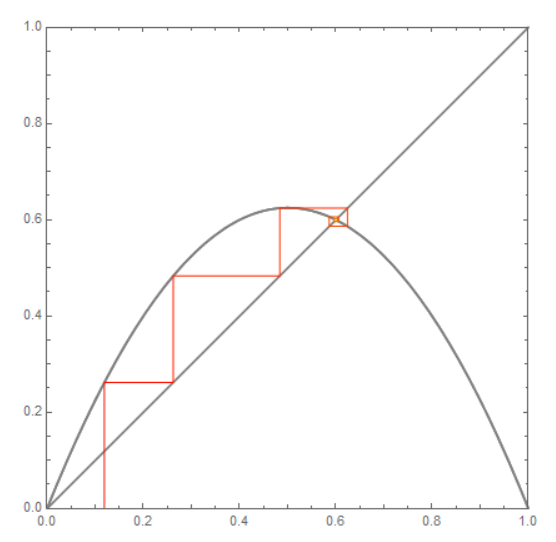
\includegraphics[width=0.24\textwidth]{img/25.png}
    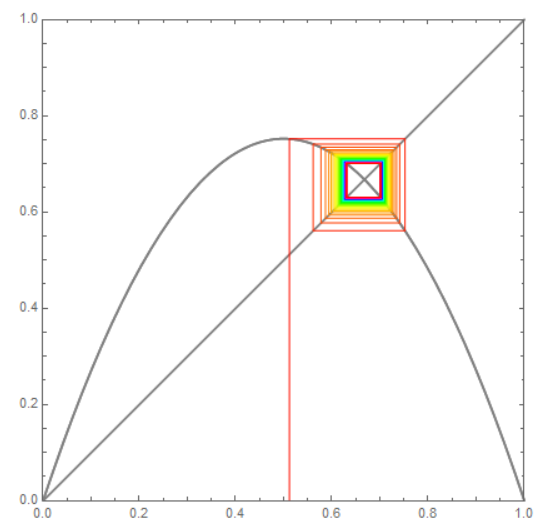
\includegraphics[width=0.24\textwidth]{img/3.png}
    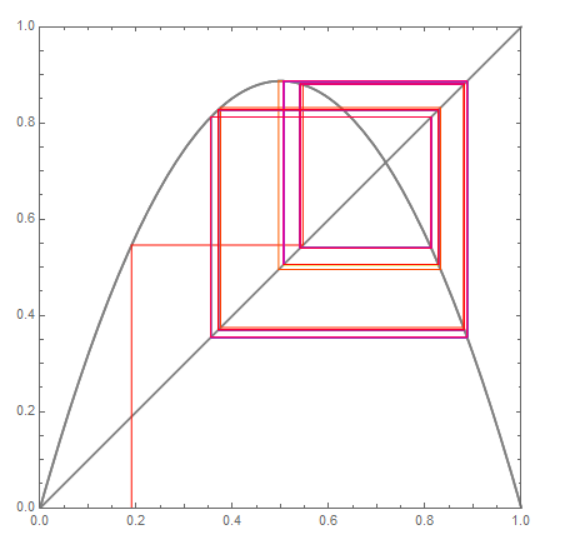
\includegraphics[width=0.24\textwidth]{img/355.png}
    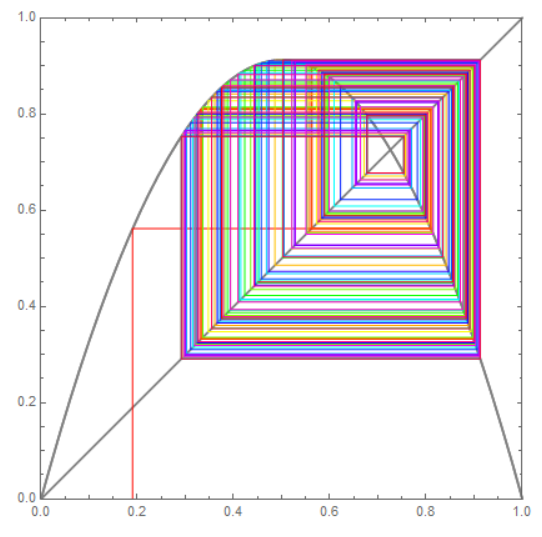
\includegraphics[width=0.24\textwidth]{img/365.png}
    \caption{Эволюция динамической системы при характерных значениях параметра}
    \label{fig:lbl}
\end{figure}
Для данного отображения в \textit{Python} была рассчитана зависимость показателя Ляпунова от параметра. Результат визуализации в представлен на рис. \ref{fig:exp}. Заметны характерные окна периодичности (см. переход к турбулентности через перемежаемость).

Стоит заметить общность использованного подхода. Так же была расчитана аналогичная зависимость для отображения Гаусса, характеризуемого двумя параметрами. Цветом показаны значения показателя Ляпунова (см. рис. \label{fig:exp}).

\begin{figure}[h]
\begin{minipage}[t]{0.49\linewidth}
        \centering
        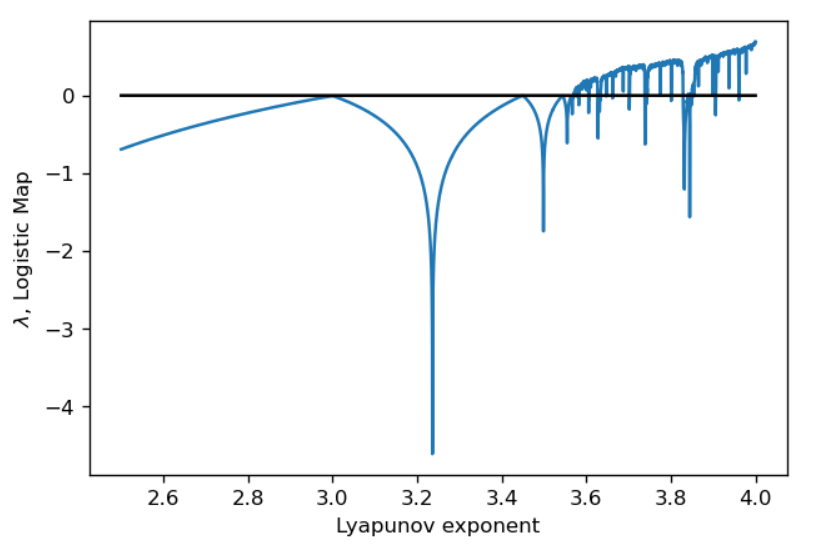
\includegraphics[width=\linewidth]{img/lyap_exp.png}
\end{minipage}
\hfill
\begin{minipage}[t]{0.49 \linewidth}
        \centering
        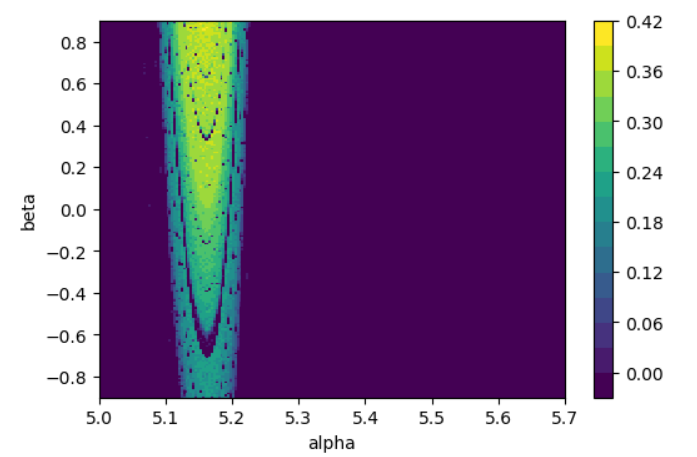
\includegraphics[width=\linewidth]{img/Gauss_map.png}
\end{minipage}
        \caption{Численный расчёт показателя Ляпунова для логистического отображения и отображения Гаусса}
        \label{fig:exp}
\end{figure}

Отдельного упоминания, бесспорно заслуживает теория развитой турбулентности, особенноработы \textit{А. Н. Колмоговроа (1941)}, \textit{А. М. Обухова (1941)}, но в связи с ограничениями по времени и некоторой отстраненностью темы она, к сожалению, была оставлена за рамками этой работы.   